In this chapter lies the most important piece of information: data and interpretation of said data. The first section (section \ref{sec:calib}) first outlined how to convert the data that the load cell actually records into the data that is relevant to this thesis. Section \ref{sec:optimiseresult} is the answer to the first objective of this thesis outlined in section \ref{sec:2}, which is what structural configuration yields the most optimum thrust. The next sections will seek to explain why and how the thrust is produced and the effect of flexibility to the generated thrust.\par
\section{Preliminary Calibration}
\label{sec:calib}
Before the experiment began, it should be made clear that the load cell used in this experiment does not directly generates force data. Instead, the load cell produce voltage as a result of strain change as a load is acting to the load cell, which in turn leads to the change of electrical resistance. Following the Wheatstone bridge circuit principle, this electrical resistance change leads to the change of voltage which can be translated into the load acting on the load cell.\par
To find the relationship between acting load and voltage output, a mini experiment to calibrate the load cell was conducted. The calibration was done by applying several predetermined loads ($W_{i}$) to the load cell and measuring the resulting voltage outputs ($V_{o}$) at a predetermined signal conditioner setup, which in this case the gain was set at 500$\times$, the lowpass frequency was set at 10 Hz and the sampling rate was set at 1000 samples/second. Each of the loads was measured several times to ensure repeatability. From the resulting data sets, a simple curve fitting method can be used to find the mathematical function that relates applied load to voltage, as shown in figure \ref{fig:calibres}.
\begin{figure}[H]
    \centering
    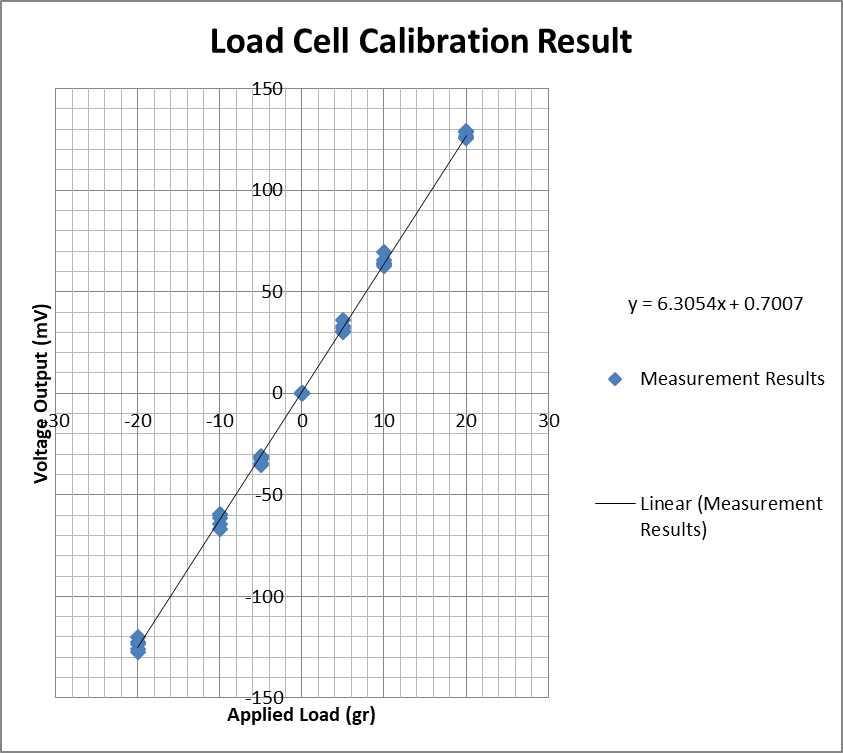
\includegraphics[scale=1]{calibres.png}
    \caption{Load cell calibration result.}
    \label{fig:calibres}
\end{figure}
From linear curve fitting method available in Excel, the relationship between voltage output and applied load can be expressed mathematically as:
\begin{equation}
    V_{o} = 6.3054W_{i} + 0.7007
    \label{eq:calibres}
\end{equation}
\section{Net Thrust Force Optimisation Result}
\label{sec:optimiseresult}
The sample points chosen to be experimentally evaluated was found through Halton sequence algorithm made by Dwianto (2015). This algorithm's output is the normalised stiffener length which served as the sample for this experiment. At each sample, the fin was flapped and moved 5 times in which each experimental runs produce 15 oscillation cycles to ensure repeatability. The net thrust force was the average of force measured in every cycle. After the sampling process is done, the resulting data sets was used to calculate the fitness function using G-SAGA and the predicted optimum value of the data was obtained. This predicted optimum value was then validated by running one more experimental run at the predicted optimum condition. Figure \ref{fig:flowchartmeth} shows the flowchart of this process.\par
\begin{figure}[H]
    \centering
    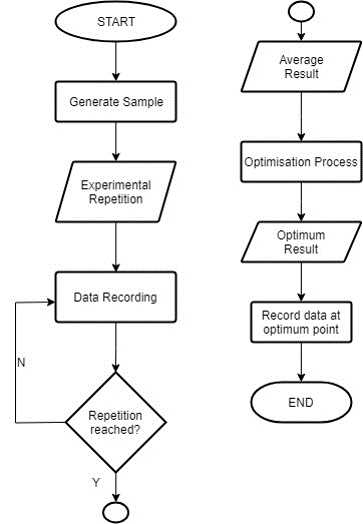
\includegraphics[scale=0.8]{flowchartmeth.png}
    \caption{Optimisation of net thrust flowchart.}
    \label{fig:flowchartmeth}
\end{figure}
Three cases were tested as part of this thesis: stiffness optimisation, stiffness and frequency optimisation, and stiffness and velocity optimisation. Those cases were chosen to observe the effect of stiffness distribution along it's chord on thrust generation and the last two cases were chosen to see the interaction between material properties (i.e. stiffness) and kinematic parameters relevant to flapping fin motion.\par
\subsection{Average Net-Thrust vs Stiffener Length}
To optimise the stiffness of the fin panel, force measurement experiment on a towing tank was conducted on the fin panel. As explained in chapter 3, the stiffness of the fin panel can be adjusted by varying the stiffener length that is embedded in the fin panel. The kinematic parameters that was kept as constant were frequency (1 Hz), amplitude (15$^{0}$), and forward velocity (1 cm/s) while the specimen's stiffness was varied by changing the length of the wire that acted as the stiffener. Figures \ref{fig:charteachrun} and \ref{fig:chartensemble} shows the result of this process.\par
\begin{figure}[H]
    \centering
    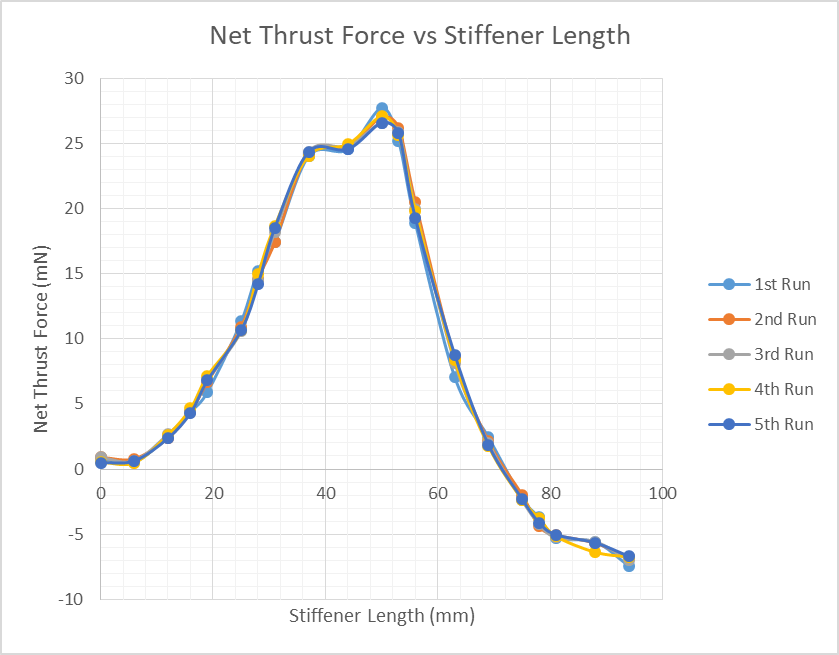
\includegraphics[scale=0.8]{chart_eachrun.png}
    \caption{Net Thrust Force vs Stiffener Length at each experimental runs.}
    \label{fig:charteachrun}
\end{figure}
\begin{figure}[H]
    \centering
    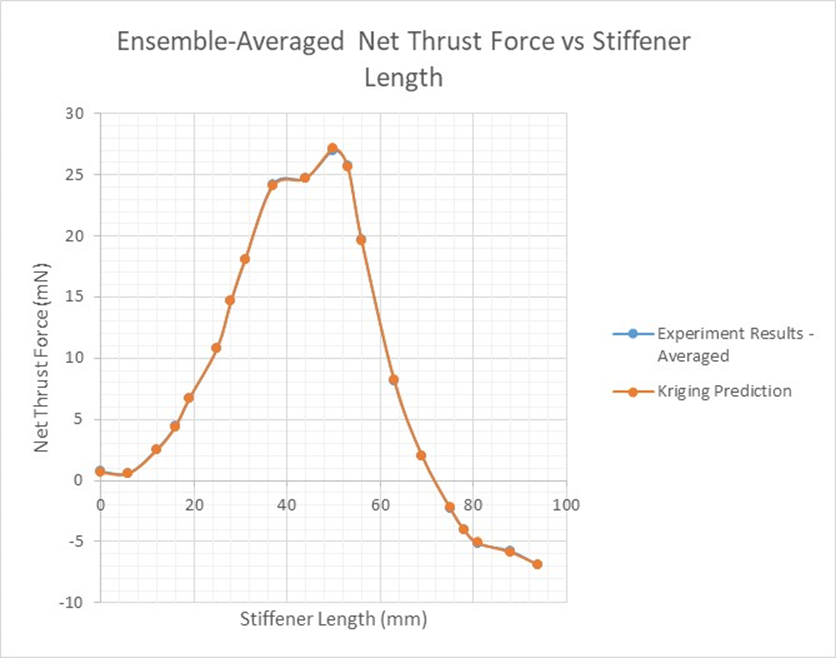
\includegraphics[scale=0.8]{chart_ensemble.png}
    \caption{Ensemble-Averaged Net Thrust Force vs Stiffener Length at each experimental runs.}
    \label{fig:chartensemble}
\end{figure}
Figure \ref{fig:charteachrun} depicts the experimental result over 5 times experimental runs and figure \ref{fig:chartensemble} represents the ensemble-averaged thrust from every experimental runs. From those figures it can be seen that neither the stiffest nor the most flexible fin produce the largest thrust. Instead, it is almost right in the middle, where 50\% wire length produce the largest thrust. It should be noted, however that the predicted thrust from genetic algorithm may very slightly differ from the true experimental result conducted at the exact same stiffener length value. The detailed numbers can be seen in table \ref{tab:tableresult} in which the disrepancies between predicted and true thrust value is almost negligible, also shown in relative error chart with respect to each population depicted in figure \ref{fig:errorfre}. Relative error denoted by $\epsilon$ (Eq. \ref{eq:relerror}) was chosen to quantify the disrepancy between kriging prediction and real experimental result.
\begin{equation}
    \epsilon = 100\% \times \left\lvert 1 - \frac{F_{kriging}}{F_{real}}\right\rvert
    \label{eq:relerror}
\end{equation}
\begin{table}[H]
\centering
\caption{Comparison table between kriging ensembled-averaged thrust force and kriging prediction.}
\vspace{5pt}
\begin{tabular}{|r|r|r|r|r|} 
\hline
No & \begin{tabular}[c]{@{}l@{}}Stiffener Length\\(mm) \end{tabular} & \begin{tabular}[c]{@{}l@{}}Ensemble Average\\(mN)~\end{tabular} & \begin{tabular}[c]{@{}l@{}}Kriging Prediction\\(mN)\\ \end{tabular} & \begin{tabular}[c]{@{}l@{}}Error\\(\%) \end{tabular}  \\ 
\hline
1  & 94                                                              & -7                                                              & -7                                                                  & 0.48                                                  \\ 
\hline
2  & 88                                                              & -6                                                              & -6                                                                  & 1.69                                                  \\ 
\hline
3  & 81                                                              & -5                                                              & -5                                                                  & 1.05                                                  \\ 
\hline
4  & 78                                                              & -4                                                              & -4                                                                  & 0.44                                                  \\ 
\hline
5  & 75                                                              & -2                                                              & -2                                                                  & 1.43                                                  \\ 
\hline
6  & 69                                                              & 2                                                               & 2                                                                   & 2.04                                                  \\ 
\hline
7  & 63                                                              & 8                                                               & 8                                                                   & 1.21                                                  \\ 
\hline
8  & 56                                                              & 20                                                              & 20                                                                  & 0.17                                                  \\ 
\hline
9  & 53                                                              & 26                                                              & 26                                                                  & 0.21                                                  \\ 
\hline
10 & 50                                                              & 27                                                              & 27                                                                  & 0.50                                                  \\ 
\hline
11 & 44                                                              & 25                                                              & 25                                                                  & 0.07                                                  \\ 
\hline
12 & 37                                                              & 24                                                              & 24                                                                  & 0.52                                                  \\ 
\hline
13 & 31                                                              & 18                                                              & 18                                                                  & 0.31                                                  \\ 
\hline
14 & 28                                                              & 15                                                              & 15                                                                  & 0.22                                                  \\ 
\hline
15 & 25                                                              & 11                                                              & 11                                                                  & 0.14                                                  \\ 
\hline
16 & 19                                                              & 7                                                               & 7                                                                   & 0.88                                                  \\ 
\hline
17 & 16                                                              & 4                                                               & 4                                                                   & 1.42                                                  \\ 
\hline
18 & 12                                                    & 3                                                               & 2                                                                   & 2.71                                                  \\ 
\hline
19 & 6                                                               & 1                                                               & 1                                                                   & 6.81                                                  \\ 
\hline
20 & 0                                                               & 1                                                            & 1                                                                   & 11.26                                                 \\
\hline
\end{tabular}
\label{tab:tableresult}
\end{table}
\begin{figure}[H]
    \centering
    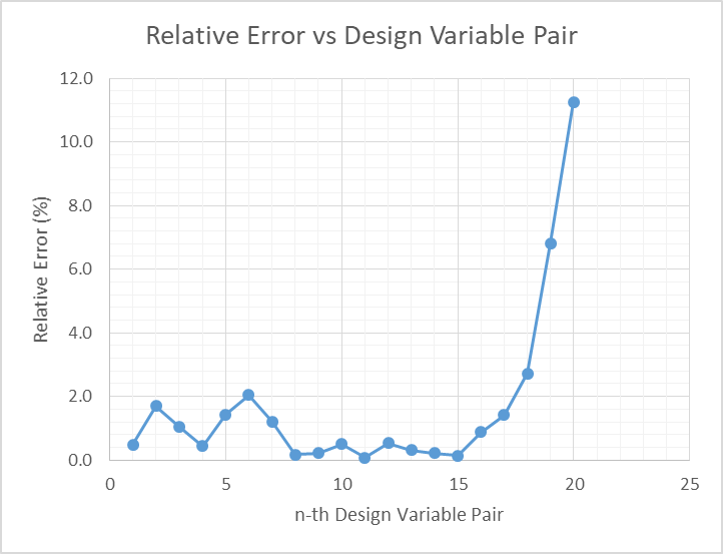
\includegraphics[scale=0.8]{errorstiff.png}
    \caption{Relative Error vs n-th population.}
    \label{fig:errorfre}
\end{figure}
To better understand what happened at each fin, the instantaneous thrust force at three flexibility conditions were presented in figure \ref{fig:chartinstant}. From this figure, it is obvious that the maximum net thrust force produced by fin with 50-50 flexibility produced the highest peak thrust with no force less than zero i.e no drag was present during the motion. However, fully-flexible or fully-stiff fins are not without merit. From the same graph, it can be observed that fully-flexible fin took less time to reached it's peak compared to the fully-stiff fin, the drawback is that while it may be beneficial to increase acceleration, the duration in which the flapping motion produce thrust is less to that of the fully-stiff fin where although it took longer for the fin to reach it's peak, the fin can maintain it's thrust for longer period of time. The same observation was made by Aiello et al. (2018) where it is stated that fish species with stiffer fin tend to produce thrust at longer period of time while flexible fin produce more acceleration at the cost of the fin's propulsion duration.
\label{sec:forceinstant}
\begin{figure}[H]
    \centering
    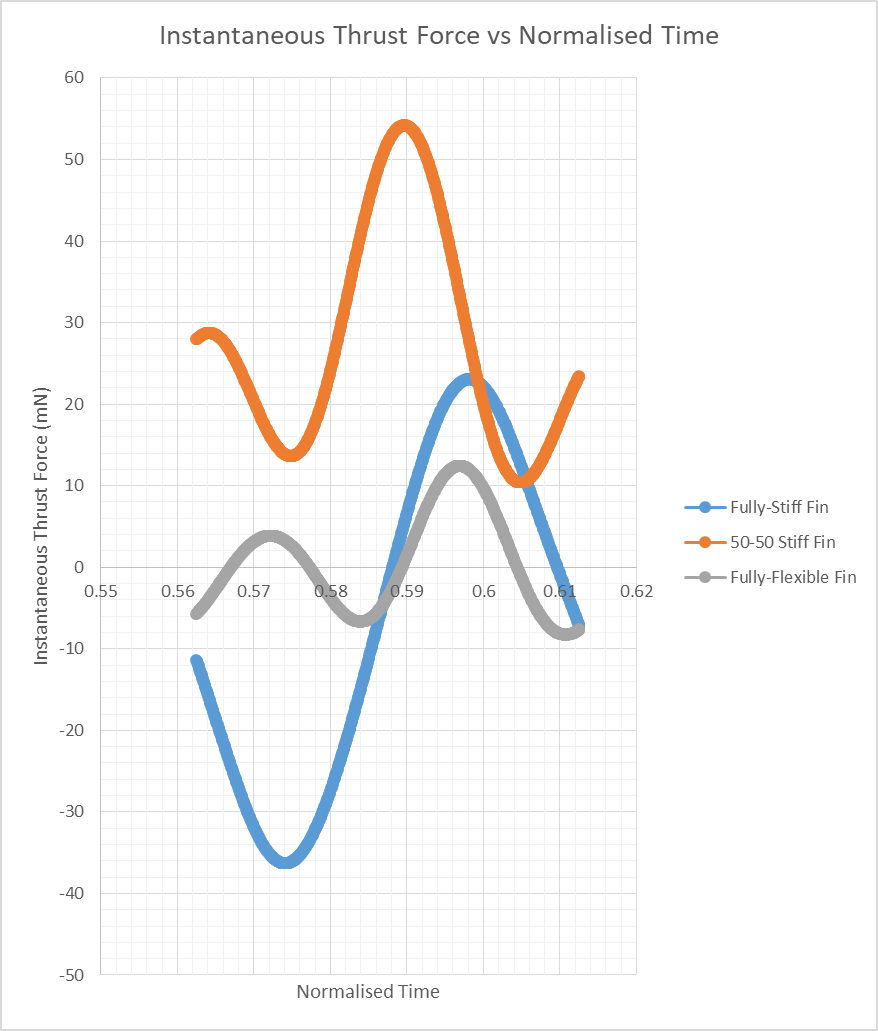
\includegraphics[scale=0.8]{chart_instant.png}
    \caption{Instantaneous Thrust Force vs normalised time.}
    \label{fig:chartinstant}
\end{figure}
\subsection{Average Net-Thrust vs Stiffener Length and Frequency Pair}
In this case, a pair of design variable was tested to find the produced thrust. Stiffener length was chosen from fully-stiff to fully-flexible and the frequency was varied from 0.5 Hz to 2 Hz. This frequency range was chosen due to the fact that the higher the frequency, the servo may not produce the same flapping amplitude as the servo ability to flap the fin was hampered by the fin's own weight. The fin velocity was kept constant at 1 cm/s and the amplitude was also kept constant at 15$^{0}$. This kinematic parameters corresponds to Strouhal number in the range of 0.15 to 0.52.\par
\begin{figure}[H]
    \centering
    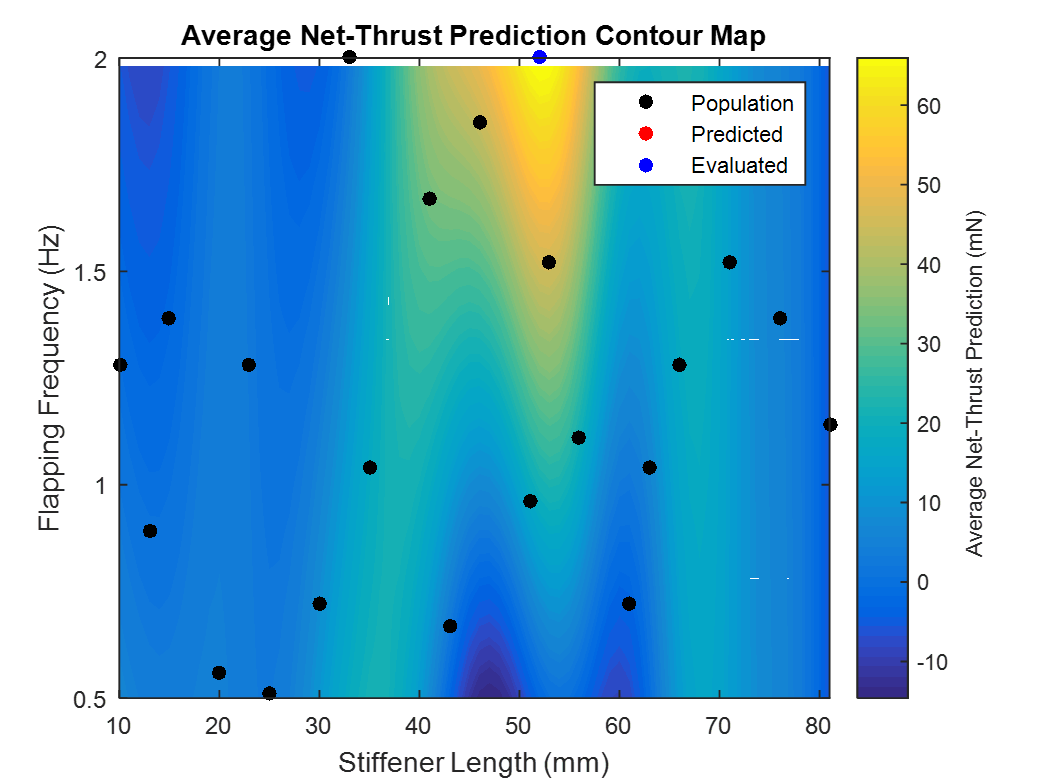
\includegraphics[scale=0.8]{chart_fre.png}
    \caption{Average Net-Thrust Force wrt Stiffener Length and Frequency Contour Map.}
    \label{fig:chart_fre}
\end{figure}
Figure \ref{fig:chart_fre} is the contour maps obtained through kriging interpolation through 21 evaluation at each population denoted by black dots. Through the algorithm, it was obtained that the optimum net-thrust was produced when the stiffness was at 52 mm flapping at 2 Hz frequency. It was predicted that the thrust will produce 67.78 mN. To check whether the prediction was true or not, an experiment was run at the predicted optimum condition which yield 68 mN net-thrust, making the relative error very small at 0.4\%, which indicates that the kriging prediction accurately predicts the average net-thrust given the stiffener length and flapping frequency. The detailed result of each population evaluation is expressed in table \ref{tab:tableresultfre} and the relative error graph can be seen in figure \ref{fig:errorfre}.
\begin{table}[H]
\centering
\caption{Comparison table between kriging ensembled-averaged thrust force and kriging prediction -- stiffness and flapping frequency combination.}
\vspace{5pt}
\begin{tabular}{|l|l|l|l|l|l|} 
\hline
\multirow{2}{*}{No} & \multicolumn{2}{c|}{Sample}                                                                                                       & \multicolumn{2}{c|}{\begin{tabular}[c]{@{}l@{}}Net-Thrust Average\\(mN) \end{tabular}} & \multirow{2}{*}{\begin{tabular}[c]{@{}l@{}}Relative Error\\(\%)~\end{tabular}}  \\ 
\cline{2-5}
                    & \begin{tabular}[c]{@{}l@{}}Stiffener Length\\(mm)\end{tabular} & \begin{tabular}[c]{@{}l@{}}Flapping Frequency\\(mN)\end{tabular} & Evaluated & Predicted                                                                   &                                                                                 \\ 
\hline
1                   & 81                                                             & 1.14                                                             & -6        & -6                                                                          & 6.6                                                                             \\ 
\hline
2                   & 76                                                             & 1.39                                                             & 6         & 6                                                                           & 6.0                                                                             \\ 
\hline
3                   & 71                                                             & 1.52                                                             & 14        & 14                                                                          & 0.0                                                                             \\ 
\hline
4                   & 66                                                             & 1.28                                                             & 18        & 18                                                                          & 2.2                                                                             \\ 
\hline
5                   & 63                                                             & 1.04                                                             & 7         & 7                                                                           & 1.1                                                                             \\ 
\hline
6                   & 61                                                             & 0.72                                                             & -3        & -3                                                                          & 10.9                                                                            \\ 
\hline
7                   & 56                                                             & 1.11                                                             & 21        & 21                                                                          & 0.9                                                                             \\ 
\hline
8                   & 53                                                             & 1.52                                                             & 46        & 46                                                                          & 0.7                                                                             \\ 
\hline
9                   & 52                                                             & 2.00                                                             & 68        & 68                                                                          & 0.3                                                                             \\ 
\hline
10                  & 51                                                             & 0.96                                                             & 17        & 17                                                                          & 2.4                                                                             \\ 
\hline
11                  & 46                                                             & 1.85                                                             & 44        & 44                                                                          & 0.2                                                                             \\ 
\hline
12                  & 43                                                             & 0.67                                                             & 3         & 3                                                                           & 1.5                                                                             \\ 
\hline
13                  & 41                                                             & 1.67                                                             & 33        & 33                                                                          & 0.2                                                                             \\ 
\hline
14                  & 35                                                             & 1.04                                                             & 18        & 18                                                                          & 0.4                                                                             \\ 
\hline
15                  & 33                                                             & 2.00                                                             & 3         & 3                                                                           & 8.5                                                                             \\ 
\hline
16                  & 30                                                             & 0.72                                                             & 9         & 9                                                                           & 4.0                                                                             \\ 
\hline
17                  & 25                                                             & 0.51                                                             & 3         & 3                                                                           & 2.4                                                                             \\ 
\hline
18                  & 23                                                             & 1.28                                                             & 3         & 3                                                                           & 4.3                                                                             \\ 
\hline
19                  & 20                                                             & 0.56                                                             & 5         & 5                                                                           & 1.3                                                                             \\ 
\hline
20                  & 15                                                             & 1.39                                                             & -2        & -2                                                                          & 2.4                                                                             \\ 
\hline
21                  & 13                                                             & 0.89                                                             & 1         & 1                                                                           & 17.8                                                                            \\ 
\hline
22                  & 10                                                           & 1.28                                                             & 0         & 0                                                                           & 100.0                                                                           \\
\hline
\end{tabular}
\label{tab:tableresultfre}
\end{table}
\begin{figure}[H]
    \centering
    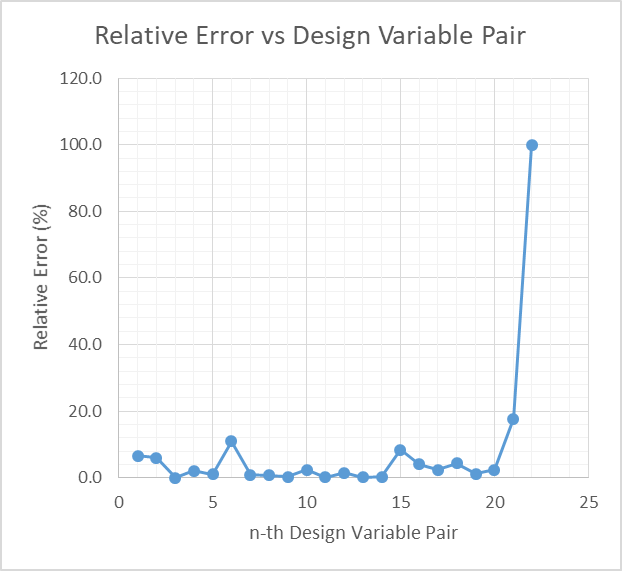
\includegraphics[scale=0.8]{errorfre.png}
    \caption{Relative Error vs n-th population -- Stiffness and Flapping Frequency Combination.}
    \label{fig:errorfre}
\end{figure}
From the relative error graph it can be seen that the kriging prediction error never exceeds 10\%, except at 22nd sample pair. This isn't to say that the kriging prediction is not globally accurate, rather the compared value (the denominator in the relative error calculation) is very close to zero, resulting in very large result, eventhough it was demonstrated that the disrepancy between the predicted average net-thrust value with the measured value is very small.
\subsection{Average Net-Thrust vs Stiffener Length and Velocity Pair}
Similar with the second case, a pair of design variable was tested to find the produced thrust. This time, the chosen kinematics parameter was forward velocity. Again, stiffener length was chosen from fully-stiff to fully-flexible while the velocity was varied from 0.15 cm/s to 4 cm/s. This velocity range was chosen to find the largest Strouhal number range possible given the experimental setup, as the faster the velocity, the more time it took to obtain 15 oscillation cycles, which means the displacement needed is also larger which was bounded by the length of the experimental setup. The fin frequency was kept constant at 1 Hz and the amplitude was also kept constant at 15$^{0}$. This kinematic parameters corresponds to Strouhal number in the range of 0.07 to 1.85.\par
\begin{figure}[H]s
    \centering
    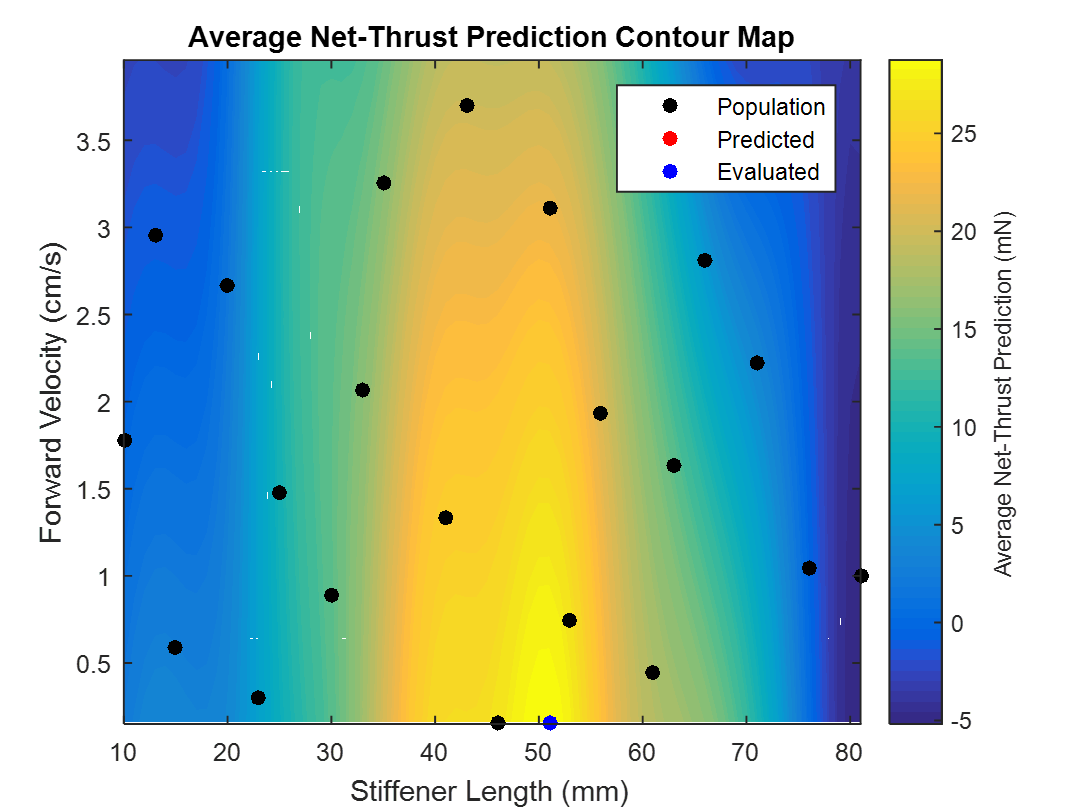
\includegraphics[scale=0.8]{chart_velo.png}
    \caption{Average Net-Thrust Force wrt Stiffener Length and Velocity Contour Map.}
    \label{fig:chart_velo}
\end{figure}
Figure \ref{fig:chart_velo} is the contour maps obtained through kriging interpolation through 21 evaluation at each population denoted by black dots. Through the algorithm, it was obtained that the optimum net-thrust was produced when the stiffness was at 51 mm moving forward at 0.16 cm/s and the predicted average net-thrust was 29.08 mN while the measured average net-thrust at the predicted optimum condition was 29 mN, resulting in an insignificant relative error: 0.3\%. This implies that the kriging prediction accurately predicts the average net-thrust given the stiffener length and forward velocity. The detailed result of each population evaluation is expressed in table \ref{tab:tableresultvelo} and the relative error graph can be seen in figure \ref{fig:errorvelo}.
\begin{table}[H]
\centering
\caption{Comparison table between kriging ensembled-averaged thrust force and kriging prediction -- stiffness and forward velocity combination.}
\vspace{5pt}
\begin{tabular}{|l|l|l|l|l|l|} 
\hline
\multirow{2}{*}{No} & \multicolumn{2}{c|}{Sample}                                                                                                       & \multicolumn{2}{c|}{\begin{tabular}[c]{@{}l@{}}Net-Thrust Average\\(mN) \end{tabular}} & \multirow{2}{*}{\begin{tabular}[c]{@{}l@{}}Relative Error\\(\%)\end{tabular}}  \\ 
\cline{2-5}
                    & \begin{tabular}[c]{@{}l@{}}Stiffener Length\\(mm)\end{tabular} & \begin{tabular}[c]{@{}l@{}}Forward Velocity\\(cm/s)\end{tabular} & Evaluated & Predicted                                                                   &                                                                                 \\ 
\hline
1                   & 81                                                             & 1.00                                                             & -5        & -5                                                                          & 2.4                                                                             \\ 
\hline
2                   & 76                                                             & 1.04                                                             & 0         & 0                                                                           & 100.0                                                                           \\ 
\hline
3                   & 71                                                             & 2.22                                                             & 4         & 4                                                                           & 3.4                                                                             \\ 
\hline
4                   & 66                                                             & 2.81                                                             & 6         & 6                                                                           & 5.8                                                                             \\ 
\hline
5                   & 63                                                             & 1.63                                                             & 14        & 14                                                                          & 0.4                                                                             \\ 
\hline
6                   & 61                                                             & 0.44                                                             & 18        & 18                                                                          & 1.2                                                                             \\ 
\hline
7                   & 56                                                             & 1.93                                                             & 21        & 21                                                                          & 0.8                                                                             \\ 
\hline
8                   & 53                                                             & 0.74                                                             & 27        & 27                                                                          & 0.9                                                                             \\ 
\hline
9                   & 51                                                             & 0.16                                                             & 29        & 29                                                                          & 0.3                                                                             \\ 
\hline
10                  & 51                                                             & 3.11                                                             & 22        & 22                                                                          & 1.4                                                                             \\ 
\hline
11                  & 46                                                             & 0.15                                                             & 27        & 27                                                                          & 1.6                                                                             \\ 
\hline
12                  & 43                                                             & 3.70                                                             & 20        & 20                                                                          & 0.2                                                                             \\ 
\hline
13                  & 41                                                             & 1.33                                                             & 25        & 25                                                                          & 1.0                                                                             \\ 
\hline
14                  & 35                                                             & 3.26                                                             & 16        & 16                                                                          & 3.0                                                                             \\ 
\hline
15                  & 33                                                             & 2.07                                                             & 16        & 16                                                                          & 3.1                                                                             \\ 
\hline
16                  & 30                                                             & 0.89                                                             & 14        & 14                                                                          & 3.1                                                                             \\ 
\hline
17                  & 25                                                             & 1.48                                                             & 10        & 10                                                                          & 4.6                                                                             \\ 
\hline
18                  & 23                                                             & 0.30                                                             & 7         & 7                                                                           & 1.3                                                                             \\ 
\hline
19                  & 20                                                             & 2.67                                                             & 2         & 2                                                                           & 4.8                                                                             \\ 
\hline
20                  & 15                                                             & 0.59                                                             & 3         & 3                                                                           & 4.1                                                                             \\ 
\hline
21                  & 13                                                             & 2.96                                                             & -1        & -1                                                                          & 65.8~ ~ ~ ~ ~~                                                                  \\ 
\hline
22                  & 10                                                        & 1.78                                                        & 0         & 0                                                                           & 100.0~~                                                                         \\
\hline
\end{tabular}
\label{tab:tableresultvelo}
\end{table}
\begin{figure}[H]
    \centering
    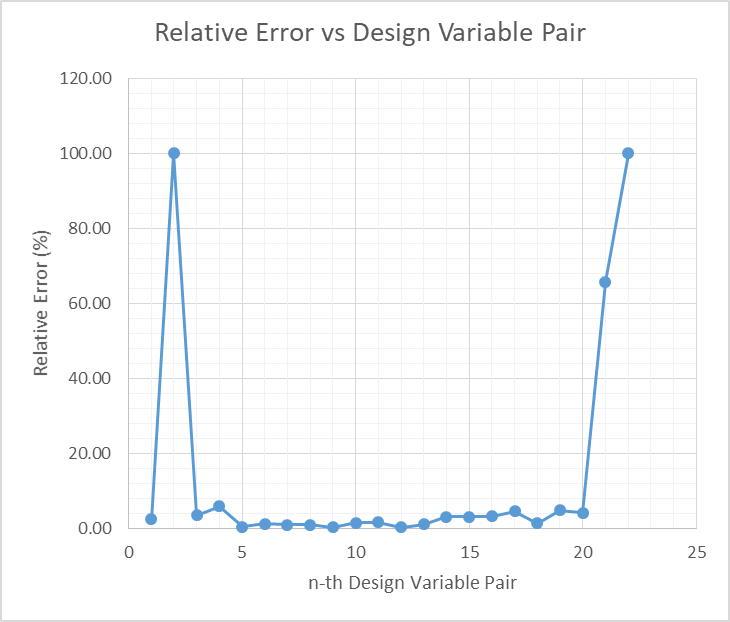
\includegraphics[scale=0.8]{errorvelo.png}
    \caption{Relative Error vs n-th population.}
    \label{fig:errorvelo}
\end{figure}
From the relative error graph it can be seen that the kriging prediction error never exceeds 10\%, except at 2nd, 21st, and 22nd sample pairs. As with the result from the frequency and stiffness measurement, the reason for this seemingly large error isn't that the kriging prediction is inaccurate, it is rather due to the compared value (the denominator in the relative error calculation) is very close to zero in the 2nd and 22nd case, and very close to -1 in the 21st sample pair case which results in a very large result, eventhough difference between the predicted average net-thrust value with the measured value is very small.
\section{Result Discussion and Analysis}
\label{sec:discuss}
Before delving deeper into the analysis of the results shown in \ref{sec:optimiseresult}, it is appropriate to first discuss whether the results obtained from the experiment is acceptable or not. One of the main difference between experimental method and computational or analytical method is that the result that one obtains may or may not be the accurate result. Unlike computational or analytical method where the same output is guaranteed given the same process and the same input, experimental method output can vary due to, for example, the existence of random noise during the experiment and the measuring instruments sensitivity. Therefore, it is important to make sure that the result obtained from experiment is the right result, or in other words, it is important to ensure the repeatability of the experimental result. The concrete value that can be used to measure the repeatability of an experiment given a set of sample $N$ of an observed variable $x$ is standard deviation depicted as $s$ (Eq. \ref{eq:stdev}) or standard deviation of the mean, represented as $s_{m}$ (Eq. \ref{eq:stdevmean}). In this thesis, the standard deviation of the mean was chosen because the value that was analysed in this thesis is the average of a value (net thrust).\par
\begin{equation}
    s = \sqrt{\frac{1}{N-1} \sum_{i=1}^N (x_i - \overline{x})^2}
    \label{eq:stdev}
\end{equation}
\begin{equation}
    s_{m} = \frac{s}{\sqrt{N}}
   \label{eq:stdevmean}
\end{equation}
\begin{table}[H]
\centering
\caption{Standard deviation of the mean for each experimental result.}
\vspace{5pt}
\begin{tabular}{|l|l|l|l|} 
\hline
\multirow{2}{*}{No} & \multicolumn{3}{l|}{\begin{tabular}[c]{@{}l@{}}Standard Deviation\\of the Mean\end{tabular}}  \\ 
\cline{2-4}
                    & Case I                             & Case II & Case II                                        \\ 
\hline
1                   & 0.14                               & 0.14    & 0.20                                           \\ 
\hline
2                   & 0.15                               & 0.20    & 0.20                                           \\ 
\hline
3                   & 0.05                               & 0.22    & 0.37                                           \\ 
\hline
4                   & 0.13                               & 0.09    & 0.24                                           \\ 
\hline
5                   & 0.07                               & 0.12    & 0.07                                           \\ 
\hline
6                   & 0.12                               & 0.18    & 0.12                                           \\ 
\hline
7                   & 0.30                               & 0.03    & 0.25                                           \\ 
\hline
8                   & 0.28                               & 0.23    & 0.08                                           \\ 
\hline
9                   & 0.16                               & 0.24    & 0.08                                           \\ 
\hline
10                  & 0.21                               & 0.11    & 0.27                                           \\ 
\hline
11                  & 0.08                               & 0.32    & 0.08                                           \\ 
\hline
12                  & \textcolor[rgb]{0.2,0.2,0.2}{0.07} & 0.21    & 0.40                                           \\ 
\hline
13                  & \textcolor[rgb]{0.2,0.2,0.2}{0.26} & 0.16    & 0.23                                           \\ 
\hline
14                  & \textcolor[rgb]{0.2,0.2,0.2}{0.18} & 0.07    & 0.08                                           \\ 
\hline
15                  & \textcolor[rgb]{0.2,0.2,0.2}{0.14} & 0.14    & 0.11                                           \\ 
\hline
16                  & \textcolor[rgb]{0.2,0.2,0.2}{0.21} & 0.14    & 0.08                                           \\ 
\hline
17                  & \textcolor[rgb]{0.2,0.2,0.2}{0.06} & 0.08    & 0.05                                           \\ 
\hline
18                  & \textcolor[rgb]{0.2,0.2,0.2}{0.06} & 0.08    & 0.16                                           \\ 
\hline
19                  & \textcolor[rgb]{0.2,0.2,0.2}{0.05} & 0.13    & 0.08                                           \\ 
\hline
20                  & \textcolor[rgb]{0.2,0.2,0.2}{0.09} & 0.04    & 0.16                                           \\
\hline
\end{tabular}
\label{tab:stddevofmean}
\end{table}
Table \ref{tab:stddevofmean} shows the standard error of the mean of each cases that was run in this thesis. Ideally, SDM close to zero is desirable as it means that the variance of the data is minimum. It is shown that the SDM of each population is less than 0.5, which leads to the conclusion that the result obtained from the experiment was indeed the right result and five experimental results are enough to obtain data point with minimum variance.\par
The changing of the fin's stiffener length (therefore it's effective stiffness) resulted in the change of thrust produced by the fin. This result is consistent with \citet{Esposito56}. From the same research, it was also shown that neither the stiffest nor the most flexible fin produce the highest thrust; instead the highest thrust was produced when the fin's stiffness was stiffer towards the leading edge up until the mid-chord and flexible from the mid-chord towards the trailing edge. Interestingly enough, this configuration holds across different kinematic parameters variation. The reason for this result was due to the nature of flapping-based thrust generation: when the fin accelerated, fluid is pushed along it's symmetrical axis and the thrust is gradually increasing as the fin goes from the extreme lateral position (i.e it's flapping amplitude). When the fin reached mid-stroke, the thrust force peaked and gradually decrease until at some point, depending on the kinematical and material properties, becomes drag \citep{Esposito56,zhushoele,akhtar}. From this argument it can then be inferred that the larger the amplitude -- therefore the lateral displacement -- the larger the thrust. This argument is backed from previous result by \citet{luqman} and \citet{hiroki} where half-stiff half-flexible fin produce the largest lateral displacement due to the difference of bending modes in various fin stiffness (see Figure \ref{fig:luqmandisp}). If the fin is fully flexible, the resulting fin shape at it's extreme amplitude is not fully deflected toward either side, instead the fin produce camber-like profile which in turn resulting in smaller lateral displacement. If the fin is fully stiff, the resulting deflection does not produce larger displacement as the fin with 50-50 stiffness.\par
\begin{figure}[H]
    \centering
    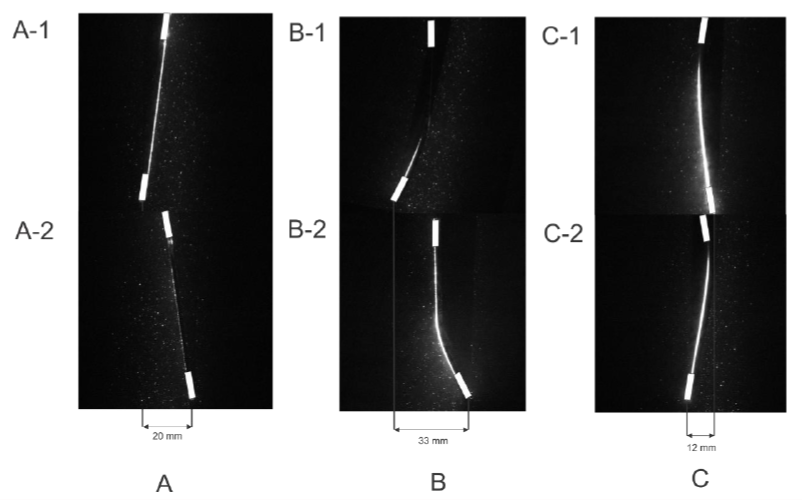
\includegraphics[scale=0.5]{luqman_disp.png}
    \caption{Real pictures captured at each extreme lateral displacement. (A) Fin number 1, (B) fin number 4, and (C) fin number 7. Upper part shows positive angle of stroke and lower one shows negative angle of stroke. Adapted from Fathurrohim (2016).}
    \label{fig:luqmandisp}
\end{figure}
\citet{aiello} also argued that this configuration (i.e stiffer at the leading edge and flexible at the trailing edge) leads to bending resistance caused by inertial and hydrodynamics forces acting on the fin where these two forces are associated with propursol reversal between the upstroke and downstroke. It is also argued that stiffened leading edge and flexible trailing edge results in propeller-like twist as a response to the torsional force, as argued by \citet{wootton} by observing that insect generates a camberline across the wing \citep{ennos}. Camber generation due to the stiffness can increase fluid dynamics efficiency and also bending resistance.\par
Frequency variation is by far the most interesting set of data. Firstly, it increased the net-thrust dramatically -- up to nearly 50\% -- which indicates that the average net-thrust change is sensitive to frequency change. Secondly, the same stiffness or frequency change does not produce predictable average net-thrust result. Eventhough 50 mm stiffener length configuration produce the largest thrust across the whole observed domain, the same cannot be said for low frequency condition where 50 mm stiffener length actually does not produce thrust at all. Rather, the lower stiffness configuration yields the most satisfying result given a particular low frequency (less than 1 Hz), as seen in figure \ref{fig:chart_surfre}.
\begin{figure}[H]
    \centering
    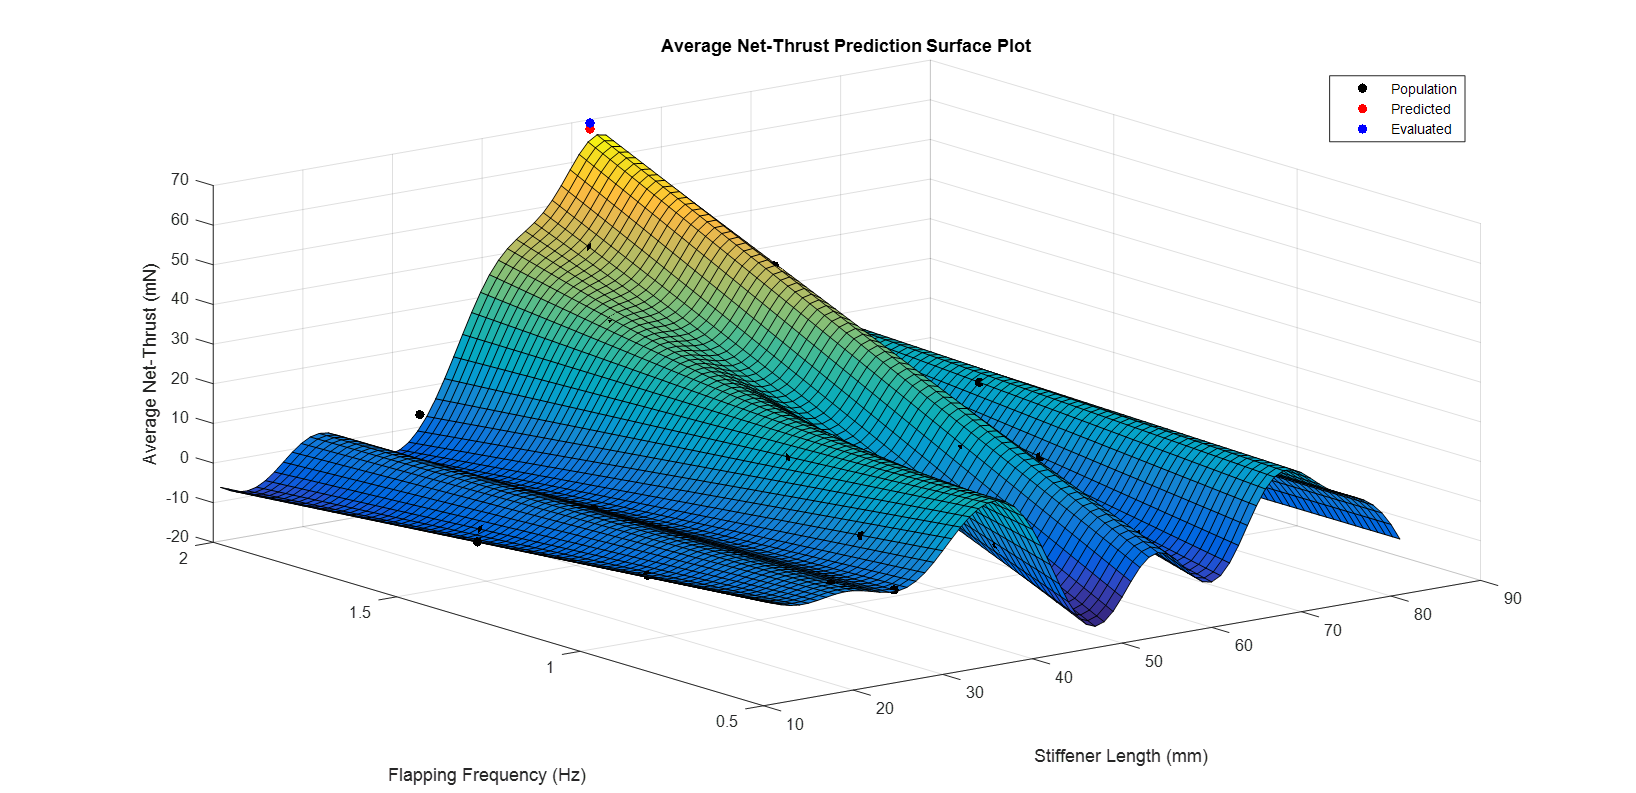
\includegraphics[scale=0.6]{chart_surfre.png}
    \caption{Average Net-Thrust Force wrt Stiffener Length and Frequency Surface Plot.}
    \label{fig:chart_surfre}
\end{figure}
This seemingly unpredictable nature of frequency change is explained by this: for each material configuration, there exist different responses for a given input. In this case, the resulting bending mode is influenced by the input frequency imposed on the fin. This different bending mode leads to smaller or larger trailing edge displacement, which directly influence the strength of the Karman vortex street behind the fin, which is the main ingredients of thrust generation through flapping mechanism. It is possible that at lower frequency, the 50 mm stiffener configuration does not produce as large of amplitude as the lower stiffness configuration, which results in lower thrust output. The same observation was made by \citet{Esposito56}, further validating this analysis.\par
Multiple interesting observations from the change of velocity variation experiment are two things: first, change of velocity and stiffness results in a somewhat uniform change in average net-thrust i.e. as the velocity decrease, the average net-thrust increase while the change of stiffness does not affect the net-thrust generation as much as the change in frequency, demonstrated in the surface plot of the average net-thrust vs flapping velocity and fin stiffness (Figure \ref{fig:chart_survelo}).
\begin{figure}[H]
    \centering
    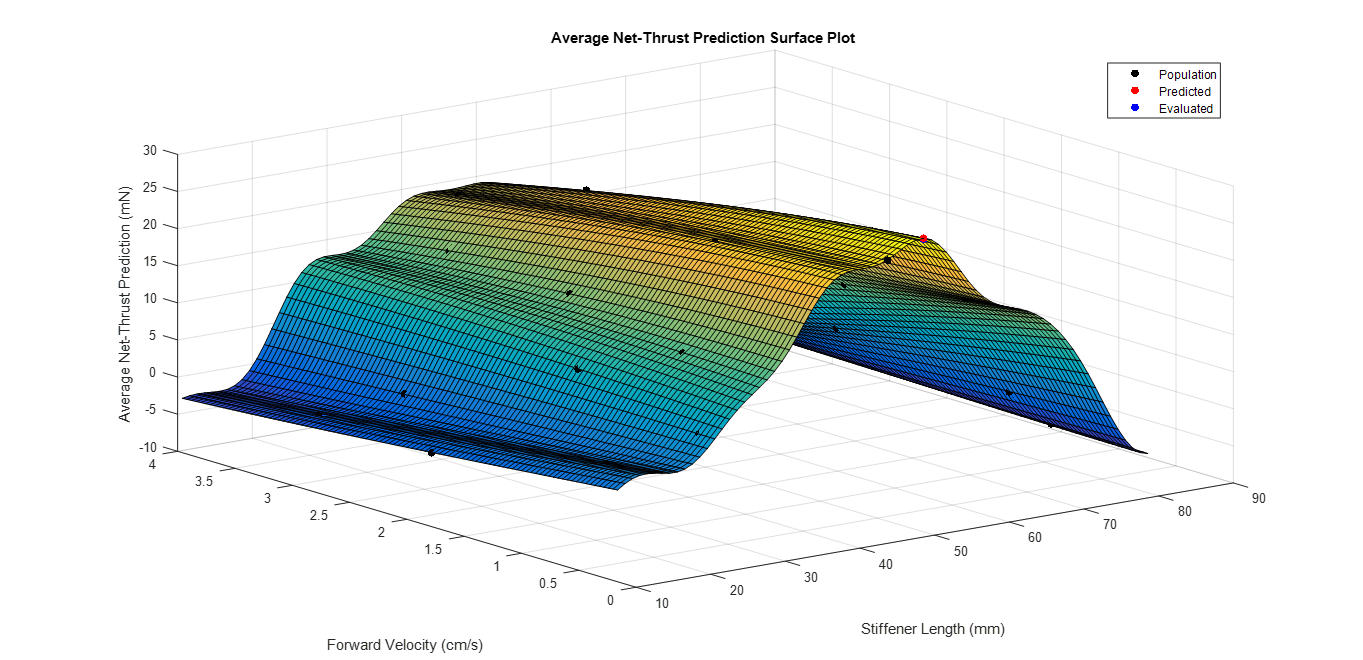
\includegraphics[scale=0.6]{chart_survelo.png}
    \caption{Average Net-Thrust Force wrt Stiffener Length and Velocity Surface Plot.}
    \label{fig:chart_survelo}
\end{figure}
This can be explained by two things: first is that aerodynamics dictates that the larger the velocity, the greater the drag force. This increase in drag force accompanying velocity increase results in the decrease in the instaneous thrust generated by the flapping fin, which leads to the decrease in the average net-thrust. Another explanation is that the nature of thrust generation through the flapping mechanism itself. From chapter II it was outlined that the thrust generated by flapping mechanism relies on the generation of reversed Karman street vortex. The reverse in vortex direction can only be achieved if the velocity combined with the flapping frequency (i.e. Strouhal number) is such that the flow around the fin produce this reverse in vortex direction. If the velocity is large enough and the frequency is small enough, the resulting vortex around the fin does not produce strong enough vortex to create a meaningful induced-velocity at the aft of the fin, which is essential to thrust generation. In some cases, as observed in the first and 21st stiffness-frequency pair, the resulting net-thrust is actually negative i.e. this configuration produces drag instead. This result arised from the fact that at this configuration, instead of the fin produced a reversed Karman vortex street, it produced an unreversed Karman vortex street which behaves similarly as if a blunt body is moving through a freestream. Another observation is that the change in velocity only results in about 6\% increase of net-thrust, compared to the nearly 150\% increase in net-thrust produced by frequency variation. This indicates that net-thrust change is not sensitive to velocity variation, as also shown by \citet{hiroki}, solidifying the analysis given in this thesis.\par